\tikzset{every picture/.style={line width=0.75pt}}

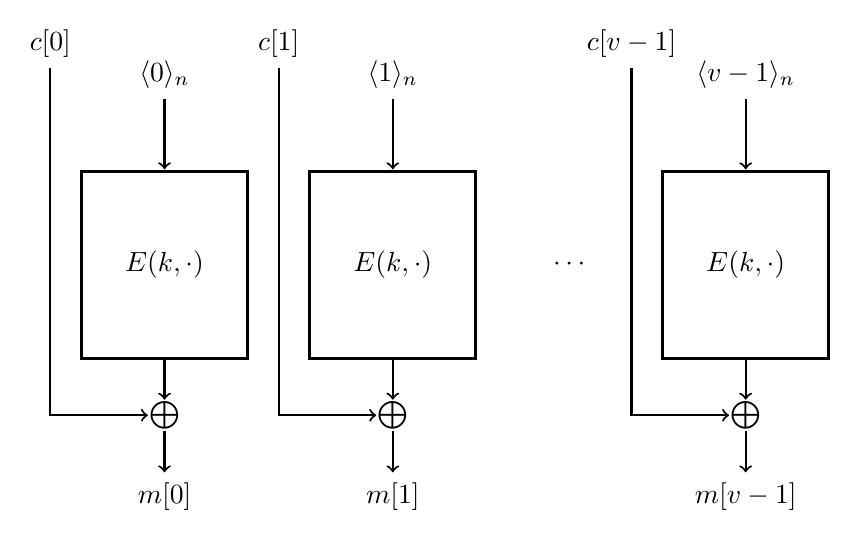
\begin{tikzpicture}[x=0.75pt,y=0.75pt,yscale=-1,xscale=1]

\draw  [line width=1.2]  (30,80) -- (110,80) -- (110,170) -- (30,170) -- cycle ;
\draw  [line width=1.2]  (140,80) -- (220,80) -- (220,170) -- (140,170) -- cycle ;
\draw  [line width=1.2]  (310,80) -- (390,80) -- (390,170) -- (310,170) -- cycle ;

\draw  [->]  (70,45) -- (70,79) ;
\draw  [->]  (180,45) -- (180,79) ;
\draw  [->]  (350,45) -- (350,79) ;
\draw  [->]  (70,170) -- (70,190) ;
\draw  [->]  (70,205) -- (70,225) ;
\draw  [->]  (180,170) -- (180,190) ;
\draw  [->]  (180,205) -- (180,225) ;
\draw  [->]  (350,170) -- (350,190) ;
\draw  [->]  (350,205) -- (350,225) ;
\draw  [->]  (15,30) -- (15,197.5) -- (62,197.5) ;
\draw  [->]  (125,30) -- (125,197.5) -- (172,197.5) ;
\draw  [->]  (295,30) -- (295,197.5) -- (342,197.5) ;

\draw (70,125) node    {$E( k,\cdot )$};
\draw (15,26.6) node [anchor=south] [inner sep=0.75pt]    {$c[ 0]$};
\draw (70.03,228.4) node [anchor=north] [inner sep=0.75pt]    {$m[ 0]$};
\draw (180,125) node    {$E( k,\cdot )$};
\draw (125,26.6) node [anchor=south] [inner sep=0.75pt]    {$c[ 1]$};
\draw (180,228.4) node [anchor=north] [inner sep=0.75pt]    {$m[ 1]$};
\draw (350,125) node    {$E( k,\cdot )$};
\draw (295,26.6) node [anchor=south] [inner sep=0.75pt]    {$c[ v-1]$};
\draw (350,228.4) node [anchor=north] [inner sep=0.75pt]    {$m[ v-1]$};
\draw (265,125) node    {$\cdots $};
\draw (70,197.5) node    {$\bigoplus $};
\draw (180,197.5) node    {$\bigoplus $};
\draw (350,197.5) node    {$\bigoplus $};
\draw (70,41.6) node [anchor=south] [inner sep=0.75pt]    {$\langle 0\rangle _{n}$};
\draw (180,41.6) node [anchor=south] [inner sep=0.75pt]    {$\langle 1\rangle _{n}$};
\draw (350,41.6) node [anchor=south] [inner sep=0.75pt]    {$\langle v-1\rangle _{n}$};

\end{tikzpicture}